\documentclass{beamer}
\usepackage{geometry}
\usepackage[english]{babel}
\usepackage[utf8]{inputenc}
\usepackage{amsmath}
\usepackage{amsfonts}
\usepackage{amssymb}
\usepackage{tikz}
\usepackage{graphicx}
\usepackage{venndiagram}

%\usepackage{pgfplots}
%\pgfplotsset{width=10cm,compat=1.9}
%\usepackage{pgfplotstable}

\setlength{\headheight}{26pt}%doesn't seem to fix warning

\usepackage{fancyhdr}
\pagestyle{fancy}
\fancyhf{}

%\rhead{\small{5 September 2018}}
\lhead{\small{BECA / Dr. Huson / 11.1 IB Math Unit 1}}

%\vspace{1cm}

\renewcommand{\headrulewidth}{0pt}


\title{Mathematics Class Slides}
\subtitle{Bronx Early College Academy}
\author{Chris Huson}
\date{5-21 September 2018}

\begin{document}

\frame{\titlepage}

%\section[Outline]{}
%\frame{\tableofcontents}

  \section{1.1 Drui}
  \frame
  {
    \frametitle{GQ: How do we define functions?}
    \framesubtitle{CCSS: HSF.IF.C.7 Analyze functions \qquad \qquad \qquad \alert{1.1}}

    \begin{block}{Do Now Handout: Algebra skills check}
    \begin{enumerate}
        \item Welcome back to school!
        \item Assigned seating: \alert{Without saying a word (!),} arrange yourself alphabetically by last name, left to right, front to back.
        \item Take out notebooks (or blank paper) \& calculator
        \item Complete handout problem set\\*
    \end{enumerate}
    \end{block}
    Lesson: Linear functions, slope, solving; vertical line test p 4-6 \\%*[5pt]
    Homework: Problem set: Function identification 1A \& 1B p. 6-7
  }
%Prepare copies of formula sheets

  \section{1.2 Drui}
  \frame
  {
    \frametitle{GQ: What are domain and range?}
    \framesubtitle{CCSS: HSF.IF.C.7 Analyze functions \qquad \qquad \qquad \qquad \qquad \qquad \qquad \alert{1.2}}

    \begin{block}{Do Now: Substitution notation}
    \begin{enumerate}
      \item Handout, IB exam problem
      \item Challenge: %2 points Aug 2017
        Verify the following Pythagorean identity for all values of $x$ and $y$:
        \[(x^2+y^2)^2=(x^2-y^2)^2+(2xy)^2\]
    \end{enumerate}
    \end{block}
    Lesson: Domain, range, slope, average rate applications\\[5pt]
    Calculator deposits \$20
    \\[5pt]
    Homework: Average rate problems (Algebra II Regents)\\
    Due: notebook, folder, calculator
  }

  \section{1.3 Drui}
  \frame
  {
    \frametitle{GQ: What is asymptotic behavior?}
    \framesubtitle{CCSS: HSF.IF.B.4 Interpret key features of functions and their graphs \hspace{\stretch{1}} \alert{1.3}}

    \begin{block}{Do Now: Graphing functions}
    \begin{enumerate}
        \item Graph \#3a, p. 12 and one other from problem 3. Use 1 cm = 1 unit
    \end{enumerate}
    \end{block}
    Review Average rate of change problem set\\ \bigskip
    Lesson: Rational functions, factoring denominators, asymptotes pp. 8-11
    \\%*[5pt]
    Homework: Function substitution, domain and range
  }

\frame
{
  \frametitle{Domain and range of a function \hspace{\stretch{1}} \alert{1.3}}
  %\framesubtitle{CCSS: HSF.IF.B.4 Interpret key features of functions and their graphs \hspace{\stretch{1}} \alert{1.3}}
  \begin{enumerate}
    \item Write down the domain and range of the function graphed\\*
    \begin{figure}[!ht]
        \centering
        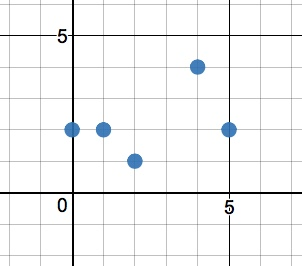
\includegraphics[width=0.35\textwidth]{discrete-domain-graph.jpeg}
    \end{figure}

    \item What is the range of this function modeling a bicycle wheel?
    \begin{figure}[!ht]
        \centering
        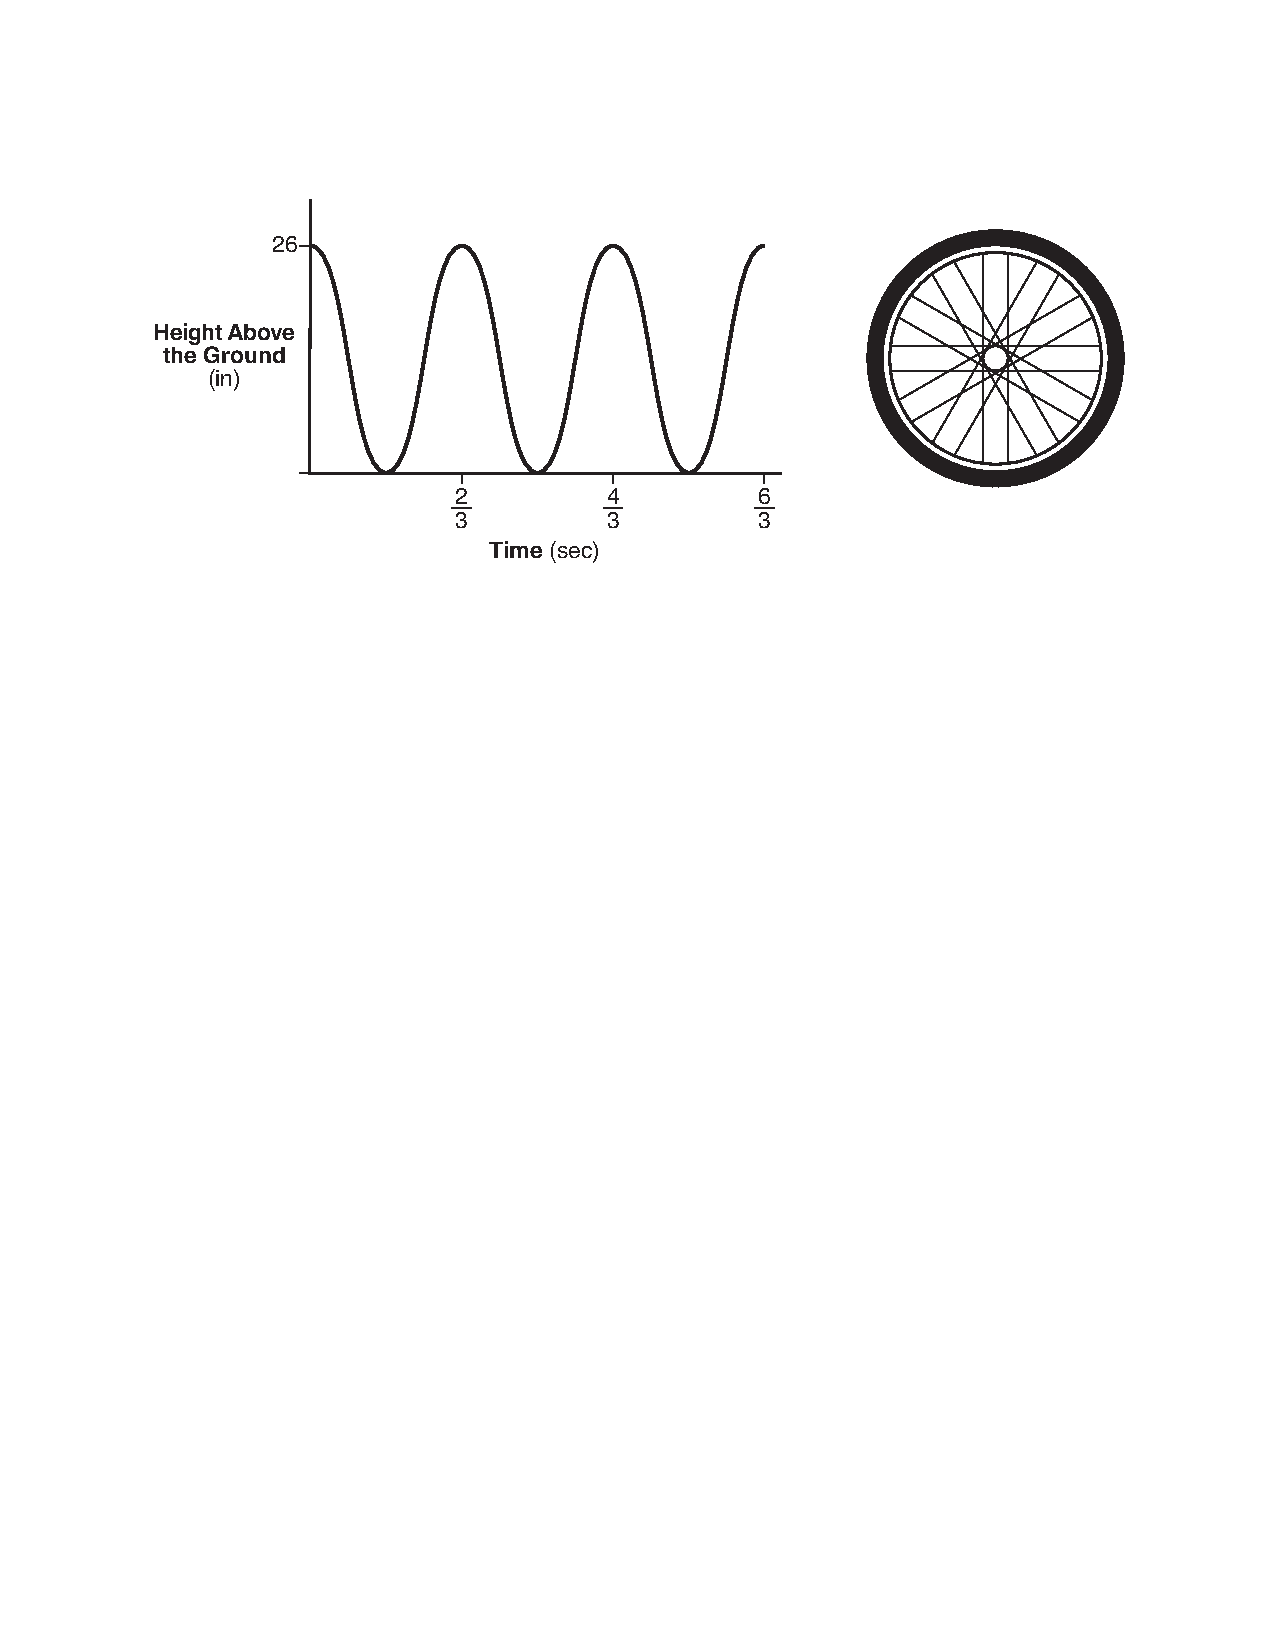
\includegraphics[width=0.70\textwidth]{sine-bike-wheel.pdf}
    \end{figure}
  \end{enumerate}
  }

\frame
{
  \frametitle{Function substitution \hspace{\stretch{1}} \alert{1.3}}
  Given $f(x)=3x+2$. What is $f(2x-1)$? \bigskip
    \begin{enumerate}
        \item Perform the substitution, putting $2x-1$ in parenthesis.\\*[20pt]
        \item Simplify, beginning each line with a leading equals sign if it is equal to the line above.\\*[40pt]
  \end{enumerate}
  }

  \section{1.4 Drui}
  \frame
  {
    \frametitle{GQ: How do we solve quadratic equations?}
    \framesubtitle{CCSS: HSF.IF.B.4 Interpret key features of functions and their graphs \hspace{\stretch{1}} \alert{1.4}}

    \begin{block}{Do Now: Factoring}
    \begin{enumerate}
        \item
        \item
    \end{enumerate}
    \end{block}
    Lesson: Factoring, setting $=0$, checking solutions, $x-$ and $y-$intercepts, vertex, axis of symmetry
    \\%*[5pt]
    Homework: Factoring practice.
  }

  \frame
  {
    \frametitle{GQ: How do we graph quadratics?}
    \framesubtitle{CCSS: HSF.IF.B.4 Interpret key features of functions and their graphs \hspace{\stretch{1}} \alert{1.4}}

    \begin{block}{Symmetry of functions, graphically and algebraically}
    \begin{enumerate}
        \item Definition: a function is \emph{even} if it can be reflected onto itself across the $y-$axix. Equivalently, iff $f(x)=f(-x)$
        \item Definition: a function is \emph{odd} if it can be reflected onto itself across the origin. Equivalently, iff $f(x)=-f(-x)$
    \end{enumerate}
    \end{block}
    Homework: Quadratics graphing
  }

  \frame
  {
    \frametitle{How do we graph quadratics?}
    \framesubtitle{CCSS: HSF.IF.B.4 Interpret key features of functions and their graphs \hspace{\stretch{1}} \alert{1.4}}

    \begin{block}{Consider the function $f(x)=-x^2+2x+3$}
    \begin{enumerate}
        \item Factor $f$ and state its zeros.
        \item Restate $f$ in vertex form. Write down the vertex as an ordered pair.
        \item Over what intervals is the function increasing, decreasing, and neither?
        \item If $f(x)$ represents the height of a diver over the domain $0 \leq x \leq 3$, interpret $f(0)$, the vertex, and $f(3)$
        \item What does the "slope" of the curve represent?
    \end{enumerate}
    \end{block}
  }


  \section{1.5 Drui}
  \frame
  {
    \frametitle{GQ: How do we calculate rates in context?}
    \framesubtitle{CCSS: HSF.IF.B.6 Calculate and interpret the rate of change of a function \hspace{\stretch{1}} \alert{1.5}}

    \begin{block}{Do Now: Sketch the function $f(x)=x^3-9x$}
      \begin{enumerate}
      \item Either factor it by hand or use a graphing calculator .
      \item "Sketch" is an IB "command term" meaning roughly show the key relationships.
      \item Label the intersections, maximum, and minimum.
      \item Add an axis caption of increasing ("++++") and decreasing ("- - - -") intervals
      \end{enumerate}
   \end{block}
    Lesson: Rates of change problem applications, graphing\\%*[5pt]
    Homework: Motion problems
  }

  \end{document}
